\documentclass[12pt,letterpaper]{article}

\usepackage{times}
\usepackage{epsfig}
\usepackage{graphicx}
\usepackage{amsmath}
\usepackage{amssymb}
\usepackage{algorithm2e}
\usepackage{mcode}
\usepackage{listings}

\newcommand{\real}{\ensuremath{\mathbb{R}}}
\newcommand{\cC}{\ensuremath{\mathbb{C}}}
\def\argmax{\mathop{\rm argmax}}
\def\argmin{\mathop{\rm argmin}}
\def\trace{\mathop{\rm trace}}

\begin{document}

\title{ Final Project: Neural Decoding using an Inhomogeneous Poisson Model}
\author{Zhengwu Zhang}
\maketitle
\thispagestyle{empty}
\section{Problem Statement}
With some data observed from animals' brain cortex, we could perform statistical analysis on these data to understand the brain mechanism and make inferences about the external behaviors. 

In this report, we have a training dataset and a testing dataset which sampled from the animals. Each of them have two variables: \textit{kin} and \textit{rate}. \textit{kin} is the kinematic state of the hand includes \textit{x-position}, \textit{y-position}, \textit{x-velocity} and \textit{y-velocity}. \textit{rate} is the spiking rates of 42 neurons, where the rate at each time is the number of spikes within $70ms$. With the training dataset we can identify the model and the apply the model into the test data to estimate the \textit{kin} with \textit{rate}. Compairation between true \textit{kin} and estimate \textit{kin} can evaluate the performance of the model. 

\section{Methodology}

\subsection{Model description}
We can use inhomogeneous Poisson process to estimate the kinematic and neurons rates. Let $x_k = [ p_{x,k}, p_{y,k},v_{x,k},v_{y,k} ]^T$ in $ \real^4 $ space denotes the hand movement of the animals, which $p_{x,k}$ denotes x-position, $ p_{y,k}$ denotes y-position, $v_{x,k}$ denotes x-velocity, $v_{y,k}$ denotes y-velocity. $y_k={y_{k,c}}$  in $\real^C$ denotes the spiking rate of $C$ neurons in the primary motor cortex at the same time. 

Assume $x_k$ follows a simple linear Gaussian transition: $x_k = A x_{k-1} + w_k$, where $w_k \in N(0,W)$. The $A$ and $W$ can be fitted in closed form using maximum likelihood estimation:

\begin{equation}
A = (\sum_{k=2}^{M}x_k x_{k-1}^T)(\sum_{k=2}^{M}x_{k-1}x_{k-1}^T)^{-1} .
\end{equation}

\begin{equation}
W = \frac{1}{M-1}(\sum_{k=2}^{M}x_k x_{k-1}^T-A \sum_{k=2}^{M}x_{k-1}x_k^T) .
\end{equation}.

For $y_{k,c},c=1,....,C$, we assume it follows a generalized linear model with an inhomogeneous poisson process condition on $x_k$: 
$$y_{k,c} \sim Poisson(\lambda_{k,c})$$, where $\lambda_{k,c} = e^{\mu_{c} + \alpha^T x_k} = e^{\theta_c^T X_k}$, $\theta_c = (\mu_c, \alpha_c^T)^T$, $X_k = (1,x_k^T)^T$. Here, $x_k$ must be centralized first. 
 
\subsection{Model Identification}

In the training set, both hand movement and neural activity are known. We could use equation (1) and (2) to calculate $A$ and $W$. After we have $A$ and $W$, we could use the MLE to estimate parameters $\theta_c = (\mu_c, \alpha_c^T)^T$. 

For each $c = 1,....,C$ assume the observations are $\{ x_k,y_{k,c}\}$. We would like to maximize the likelihood: 
\begin{equation}
L = p(y_{k,c}|x_k) = \prod_{k=1}^M p(y_{k,c}|x_k) = \prod_{k=1}^M \frac{e^{-\lambda_{k,c}(\lambda_{k,c})^{y_{k,c}}}}{y_{k,c}!}
\end{equation}

we get the log-likelihood function:
$$LL = \sum_{k=1}^{M} log(\lambda_{k,c}) - \lambda_{k,c} + const
$$
where $\lambda_{k,c} = e^{\theta_c^T X_k}$

One can use Newton-Raphson method to solve the MLE problem. The first and seconde derivatives are:
$$\frac{\partial LL}{\partial \theta_c} = \sum_{k=1}^{M} y_{k,c} X_k - e^{(\theta_c^T X_k)X_k}$$

$$\frac{\partial ^2 LL}{\partial \theta_c \partial \theta_c^T} = -\sum_{k=1}^{M} e^{(\theta_c^T X_k)X_k X_k^T}$$

The recursive update function is: $(\theta_c)_{i+1} = (\theta_c)_i - (\frac{\partial^2 LL}{\partial \theta_c \partial \theta_c^T})^{-1}_i (\frac{\partial LL}{\partial \theta_c})_i$

\subsection{Neural Decoding}

Neural Decoding is using the spiking data to infer the movement behaviors of the hand. 
Once we have the parameters of the model, we can perform neural decoding on the testing data.  We have two methods to infer the Neural decoding now: Point Process Filter and Sequential Monte Carlo Method.

\subsubsection{Point Process Filter}
Point Process Filter is based on Laplace approximation by approximate the posterior at each time using a Gaussian distribution. The recursive formula is:

$$f(x_k|y_1,...,y_k) \propto f(y_k|x_k) f(x_k| y_1,...,y_{k-1}) $$

Assume that conditioned on $x_k$, all components in $y_k$ are independent. Therefore:

$$f(y_k|x_k) = \prod_{c+1}^C {f(y_{k,c}|x_k)}$$

The algorithm of Point Process Filter can be divided into two parts: Time Update and Measurement Update.

\begin{enumerate}

\item Time update, one estimate posterior using Gaussian distribution, $$x_{k|k} = E(x_{k}|y_{1:k}),W_{k|k} = Var(x_k|y_{1:k})$$ then $f(x_k|y_{1:k-1})$ is also normally distribution. The mean is $x_{k|k-1}=E(x_k|y_{1:k-1})=A x_{k-1|k-1}$, the covariance is: 
$$W_{k|k-1} = var(x_k|y_{1:k-1})=A W_{k-1|k-1} A^T + W$$

Therefore, 
$$ f(x_k|y_1,...,y_k) \propto f(y_k|x_k) f(x_k| y_1,...,y_{k-1}) = \prod_{c=1}^C{Poisson(\lambda_{k,c})}* N(x_{k|k-1},W_{k|k-1}) $$

\item Measurement Update , take the log of the posterior and using Gaussian distribution to estimate it, we get:

$$\frac{1}{2} (x_k-x_{k|k})^T W^{-1}_{k|k} (x_k-x_{k|k}) = \frac{1}{2}  (x_k-x_{k|k-1})^T W^{-1}_{k|k-1} (x_k-x_{k|k-1}) - (\sum_{c=1}^C {y_{k,c} log \lambda_{k,c} - \lambda_{k,c}}) + c $$

Differentiate w.r.p to $x_k$ twice we get:

$$W^{-1}_{k|k} = W^{-1}_{k|k-1} + \sum_{c=1}^C{\frac{\partial \lambda_{k,c}}{\partial x_k} \alpha_c} $$

Let $x_k = x_{k|k-1}$ after the second differentiation, we have

$$W_{k|k} = (W^{-1}{k|k-1} + \sum_{c=1}^{C}{\alpha_c e^{\mu_c + \alpha^T_c x_{k|k-1}} \alpha_c^T})^{-1} $$

Let $x_k = x_{k|k-1}$ after the first differentiation,we have

$$x_{k|k} = x_{k|k-1} + W_{k|k} \sum_{c=1}^C [y_{k,c} - e^{\mu_c + \alpha^T_c x_{k|k-1}}] \alpha_c $$

\end{enumerate}

With time update parameters $W_{k|k-1}, x_{k|k-1}$ and measurement update $W_{k|k}, x_{k|k}$, we can calculate the recursive process to obtain $x_{k|k}$. 

\subsubsection {Monte Carlo Method}

Sequential Monte Carlo Methods also can dived into two parts: Prediction step and Update Step. The details of this algorithm can be found in the book. The basic form of sequential Monte Carlo algorithm is:

\begin{enumerate}
\item Genrate n samples $x_0^i \sim f(x+0).$ Set $t=0$.

\item Prediction: Generate the prediction set using: $\tilde{x}_{t+1}^i \sim f(x_{t=1}|x^i_t),i=1,2...,n.$

\item Update: Compute the weights $w^i_{t+1} = f(y_{t+1}|\tilde{x}_{t+1})$, and normalize them using $\tilde{w}^i_{t+1} = \frac{w^i_{t+1}}{\sum_{j=1}^n{w^j_{t+1}}}$. 

Estimate $\theta_{t+1}$ using $ \hat {\theta}_{t+1} = \sum_{i=1}^n{g(\tilde{x}^i_{i+1})\tilde{w}^i_{t+1}}$  

Resample from the set $\{\tilde{x}_{t+1}^1,...,\tilde{x}^n_{t+1} \}$ with probabilities $\{ \tilde{w}^1_{t+1},..., \tilde{w}^n_{t+1} \}$. 


\item Set $t=t+1$, and return to Step 2. 

\end{enumerate}

\section{Experiment results}
\subsection{Point Process Filter}

\begin{figure}
\begin{center}
\includegraphics[width=0.9\linewidth]{PointPF.eps}
\caption{Experiment Results of Point Process Filter}
\label{fig:database}
\end{center}
\end{figure}

The $R^2$ we get is: [ 0.3955 0.6542 0.4751  0.7571] w.r.t x-position, y-position, x-velocity, y-velocity. 

\subsection{Sequential Monte Carlo Method}

\begin{enumerate}


\item sample size n=20. The $R^2$ we get is: [0.0977  0.5990  0.3186   0.6854].

\begin{figure}
\begin{center}
\includegraphics[width=0.9\linewidth]{SMC20.eps}
\caption{Experiment Results of Sequential Monte Carlo Method with sample size 20}
\label{fig:database}
\end{center}
\end{figure}


\item sample size n=50. The $R^2$ we get is: [0.2726 0.6490  0.4259  0.7247].

\begin{figure}
\begin{center}
\includegraphics[width=0.9\linewidth]{SMC50.eps}
\caption{Experiment Results of Sequential Monte Carlo Method with sample size 50}
\label{fig:database}
\end{center}
\end{figure}


\item sample size n=100. The $R^2$ we get is: [0.3157  0.6326  0.4609  0.7269].

\begin{figure}
\begin{center}
\includegraphics[width=0.9\linewidth]{SMC100.eps}
\caption{Experiment Results of Sequential Monte Carlo Method with sample size 100}
\label{fig:database}
\end{center}
\end{figure}


\item sample size n=500. The $R^2$ we get is: [0.3641  0.6695  0.4792  0.7526].

\begin{figure}
\begin{center}
\includegraphics[width=0.9\linewidth]{SMC500.eps}
\caption{Experiment Results of Sequential Monte Carlo Method with sample size 500}
\label{fig:database}
\end{center}
\end{figure}

\end{enumerate}

We summarize the $R^2$ into a table.
\begin{center}
\begin{tabular} { | l | l | l | l | l | l | }
\hline
Variable & X-Position & Y-Position & X-Velocity & Y-Velocity \\ \hline
Point Proc. Filter & 0.3955 &0.6542 & 0.4751 & 0.7571 \\ \hline
Sequ. Monte Carlo(n=20) & 0.0977 & 0.5990 & 0.3186 & 0.6854\\ \hline
Sequ. Monte Carlo(n=50) & 0.2726 & 0.6490 & 0.4259 & 0.7247\\ \hline
Sequ. Monte Carlo(n=100) & 0.3157 & 0.6326 & 0.4609 & 0.7269\\ \hline
Sequ. Monte Carlo(n=500) & 0.3641 & 0.6695 & 0.4792 & 0.7526\\ \hline

\end{tabular}
\end{center}

\section{Summary}
In this report we introduce two different method to the Neural Decoding: Point Process Filter and Sequential Monte Carlo Method. From the results we can see that Point Process Filter perform better at X-Position and Y-Velocity even we use 500 samples with Sequential Monte Carlo Method. When Sequential Monte Carlo Method have fewer samples, its performance become worse and worse. 

Also the efficiency of Point Process Filter is very high. Once can finish estimation in a few seconds. But the Sequential Monte Carlo Method is not efficiency at all. It takes more then 10 mins to do the estimation with 500 samples.  (Maybe my program is very bad)

In a words, Point Process Filter is a very good tool to do this kind of estimation.

\section{Matlab Programs}

Matlab Program for Point Process Filter

  \begin{lstlisting}
  clear all;
close all;
%Final Project
load('final_train.mat');

[M,c] = size(rate);
[M,d] = size(kin);

%center data
kin = kin-ones(M,1)*mean(kin);

%with MLE to find A and W;
X_a = kin(2:M,:)';
X_b = kin(1:M-1,:)';

A = X_a*X_b'*inv(X_b*X_b');
W = (X_a-A*X_b)*(X_a-A*X_b)'/(M-1);

%Inhomogeneous Possion process
kin=[ones(M,1),kin];

for i=1:c
    %initial
    alpha_o = zeros(d+1,1);
    alpha_n = alpha_o + 1; 
    
    
    %use Newton-Raphson method to solve MLE
    while(norm(alpha_n-alpha_o)>1e-2)
        alpha_o = alpha_n;
        
        fdd=kin'*rate(:,i)-kin'*exp(kin*alpha_o); %first
        
        sdd = -kin'.*(ones(d+1, 1)* exp(kin * alpha_o)')*kin; %second;
        
        alpha_n = alpha_o - inv(sdd)*fdd;
        
    end;
    
    alpha(:,i) = alpha_n;
    
end;

%point process Filter algorithm

load ('final_test.mat');
[M,c] = size(rate);
[M,d] = size(kin);

kin = kin-ones(M,1)*mean(kin);
kin = kin';
%initial W_kt(4 by 4) and W_km(4 by 4)
W_kt(1,:,:) = eye(4);
W_km(1,:,:) = eye(4);
X_kt(:,:) = zeros(d,1);
X_km(:,:) = zeros(d,1);

Ac = alpha(2:5,:);
Muc = alpha(1,:);

for i=2:M

    %time update:
    W_kt(i,:,:) = A*squeeze(W_km(i-1,:,:))*A' + W;
    X_kt(:,i) = A*X_km(:,i-1);
    
    %measurement update;
    
    %compute second part of measurement update;
    Lp = zeros(4,4);
    
    for t=1:c
        Lp = Lp + Ac(:,t)*exp(Muc(t)+Ac(:,t)'*X_kt(:,i))*Ac(:,t)';
    end;
    
    W_km(i,:,:)=inv(inv(squeeze(W_kt(i,:,:)))+ Lp);
    
    XLp = zeros(d,1);
    
    for t=1:c
        XLp = XLp + (rate(i,t) - exp (Muc(t)+Ac(:,t)'*X_kt(:,i)))*Ac(:,t);
    end;
    
    X_km(:,i) = X_kt(:,i) + squeeze(W_km(i,:,:))*XLp;
    
end;

%Rsqure
Rsq = 1 - sum((X_km - kin).^2,2)./sum(kin.^2,2);  

% plot figure;
for i=1:d
subplot(4,1,i)
plot(1:M,X_km(i,1:M),'-.r');
hold on;
plot(1:M,kin(i,1:M));
title('True and estimated state');
legend('Estimated State','True state');
legend('boxoff');
end;

print -depsc PointF
  
  \end{lstlisting}
  
  
  
  Matlab Program for Sequential Monte Carlo

  \begin{lstlisting}
  %final project
%Sequential Monte Carlo Method;

clear all;
close all;

load final_train.mat
%model identification
[M,c] = size(rate);
[M,d] = size(kin);

%center data
kin = kin-ones(M,1)*mean(kin);

%with MLE to find A and W;
X_a = kin(2:M,:)';
X_b = kin(1:M-1,:)';

A = X_a*X_b'*inv(X_b*X_b');
W = (X_a-A*X_b)*(X_a-A*X_b)'/(M-1);

%Inhomogeneous Possion process
kin=[ones(M,1),kin];

for i=1:c
    %initial
    alpha_o = zeros(d+1,1);
    alpha_n = alpha_o + 1; 
       
    %use Newton-Raphson method to solve MLE
    while(norm(alpha_n-alpha_o)>1e-2)
        alpha_o = alpha_n;
        
        fdd=kin'*rate(:,i)-kin'*exp(kin*alpha_o); %first     
        sdd = -kin'.*(ones(d+1, 1)* exp(kin * alpha_o)')*kin; %second;
        
        alpha_n = alpha_o - inv(sdd)*fdd;        
    end;
    alpha(:,i) = alpha_n;
    
end;

Ac = alpha(2:5,:);
Muc = alpha(1,:);

load final_test.mat

[M,c] = size(rate);
[M,d] = size(kin);

%sample size
N = 500;

%generate n samples
x_e(:,:,i) = rand(4,N);

for i=2:M   
    if (mod(i,100)==0)
        display(i);
    end;
    
    %generate the prediction
    tmp = mvnrnd(zeros(4,1),W,N)';
    
    x_tilte(:,:,i) = A*squeeze(x_e(:,:,i-1))+tmp;
    
   %compute the weights 
   %..........................................
   for t=1:N
   %For each sample compute lambda first and compute the log likelihood of possion
   Loglikel = zeros(d,1);
   for x =1:c
        lambda(i,x) = exp(Muc(1,x) + Ac(:,x)'*x_tilte(:,t,i));
        Loglikel(x,1) = log(lambda(i,x))*rate(i,x)-lambda(i,x)-log(factorial(rate(i,x)));
   end;
   w(i,t) = exp(sum(Loglikel));
   end;
   %..................................................
    
   %normalize the weight;
    w_n(i,:) = w(i,:)/sum(w(i,:));
    W_n(i,:) = cumsum(w_n(i,:));
    
    %estimate theta
    theta_hat(i,:) = w_n(i,:)*squeeze(x_tilte(:,:,i))';    

    %resample
    for t = 1:N
        U = rand;
        ind = find(U-W_n(i,:)<0);
        x_e(:,t,i) = x_tilte(:,ind(1),i);
    end;
end;


kin = kin - ones(M,1)*mean(kin);
for i=1:d
    subplot(4,1,i);
    plot(1:M,kin(:,i),1:M,theta_hat(:,i),'-.r');
    title('True and estimated state');
    legend('Estimated State','True state');
    legend('boxoff');
end;

%Rsq
Rsq = 1 - sum((theta_hat' - kin').^2,2)./sum(kin'.^2,2)



  \end{lstlisting}


\end{document}